\begin{tikzpicture}%[show background grid]% every node/.style={draw,outer sep=0pt,thick}]

% SoT
\draw [fill=green,opacity=.2,text opacity=1] (-1.5,2.2) rectangle (13.0,-2.2);
\node at(6,-2.0) {\textcolor{green!20!black!100}{Stack of Task}};

% Ellispe Reference
\node[rectangle,minimum width=2cm, minimum height=1cm,draw=blue!70,fill=blue!20] (ellipseref) at (4.0,3.25) {};
\node[ellipse,draw=blue,thick,minimum width=1cm,minimum height=0.5cm] at (ellipseref) {};
\node at ([yshift=-0.8cm]ellipseref) {Reference trajectory};

% Vector Field
\node[rectangle,minimum width=2cm, text width=2cm,minimum height=1cm,draw=blue!70,fill=blue!20,align=center] (vectorfields) at (0.0,0.0) 
{Vector Field\\
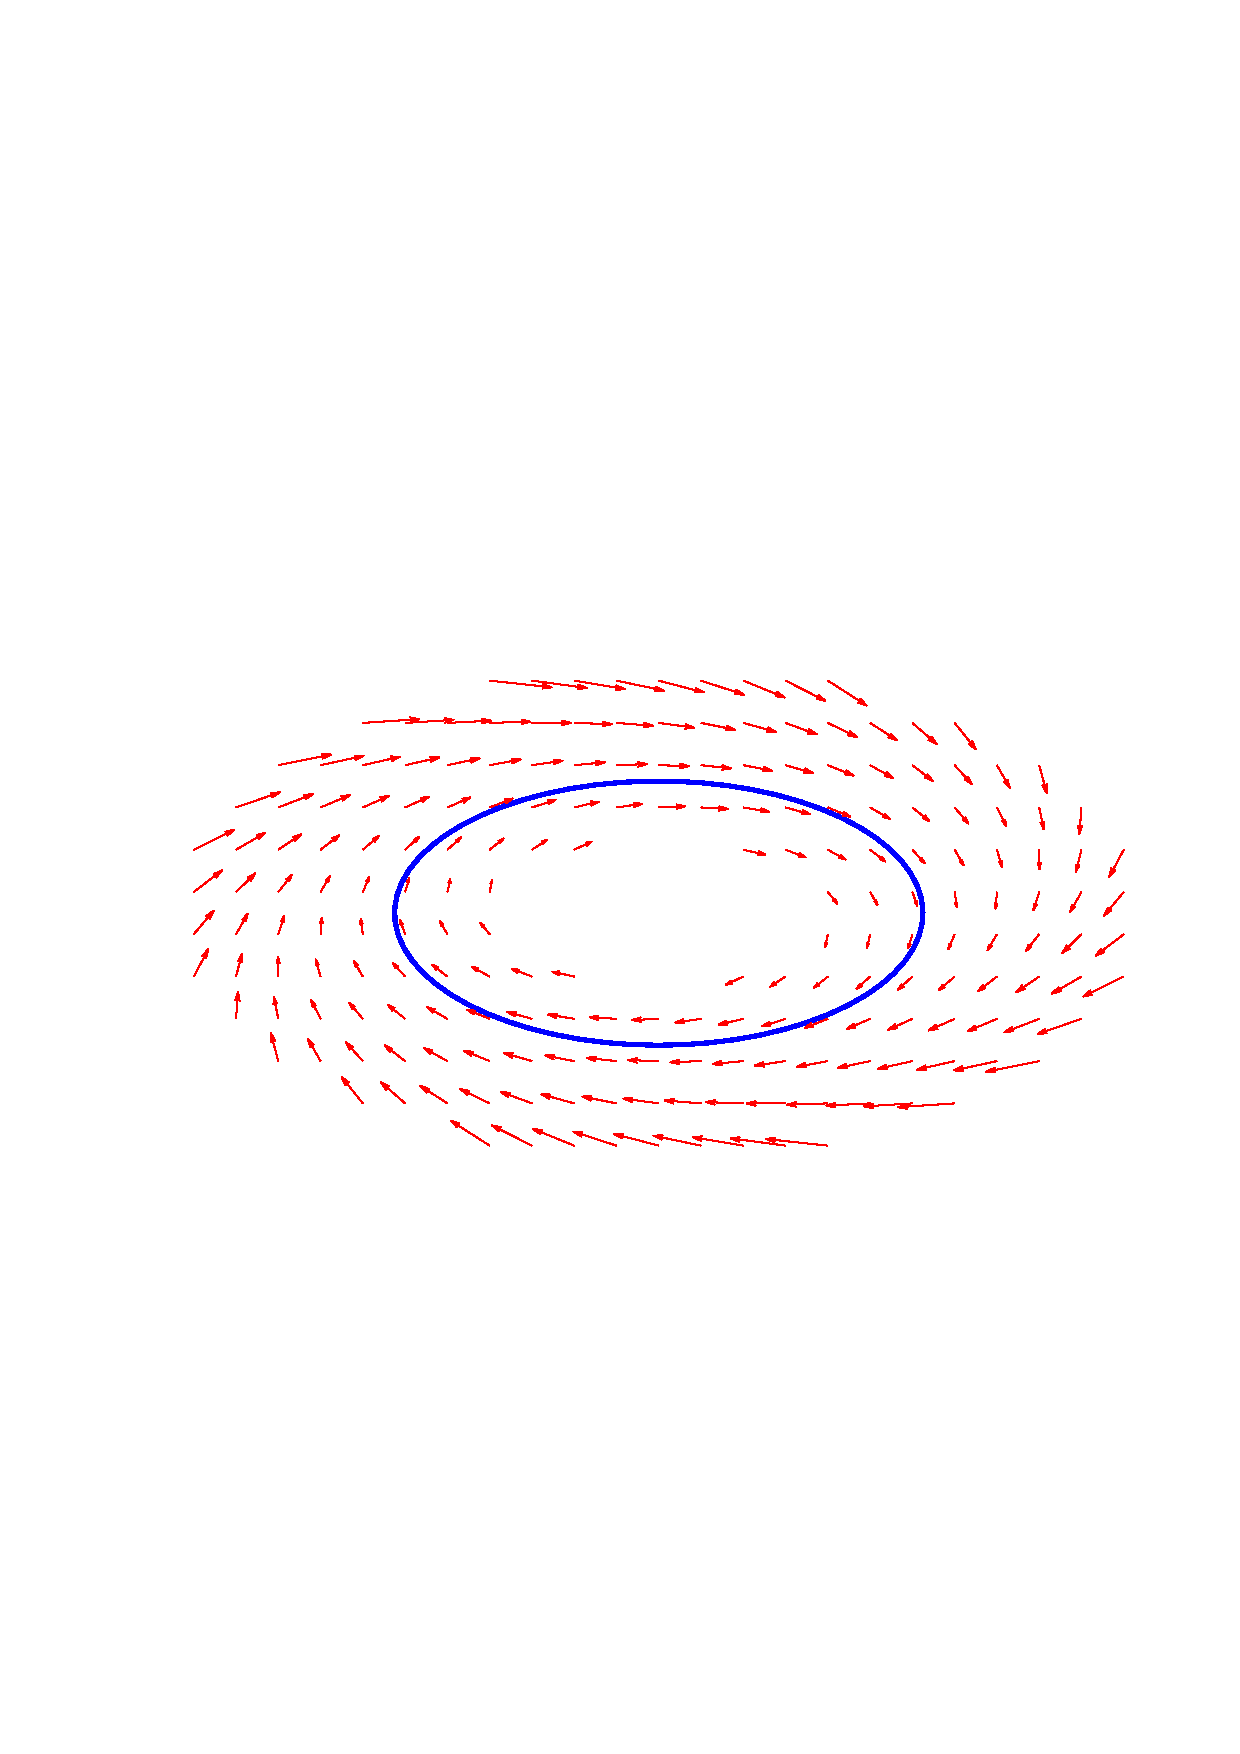
\includegraphics[scale=0.1]{./TwoThirdPowerLawApplication/figures/Fig3e_EllipseBetaThird.pdf}};
%\node at (0.0,2.5) {$\gamma,\beta$};

% Walking Pattern Generator
\node[rectangle,minimum width=2cm, minimum height=1cm,draw=blue!70,fill=blue!20]  (wpg) at (5.4,1.0) {Walking Pattern Generator};

% Task
\node[rectangle,minimum width=2cm, text width=3cm, align=center, minimum height=1cm,draw=blue!70,fill=blue!20] (ttt) at (11,1.0) 
{  Task for\\
   Trajectory\\
   Tracking};

% Solver
\node[rectangle,minimum width=2cm, text width=3cm, align=center, minimum height=1cm,draw=blue!70,fill=blue!20] (qp) at (11,-1.0) 
{ QP Solver };

% Power Law
\node[rectangle,text width=2cm,align=center,minimum width=2cm, minimum height=1cm,draw=blue!70,fill=blue!20] (powerlaw) at (3.0,-1.0) {Power Law\\$\gamma,\beta$};
\path[->,>=stealth',draw=black] (vectorfields.314)-- node[below] {$\kappa$} (powerlaw.189);
\path[->,>=stealth',draw=black] (powerlaw.170)-- node[above] {$v$} (vectorfields.325);

% Robot
\node[rectangle,minimum width=2cm, minimum height=1cm,draw=blue!70,fill=blue!20] (robot) at (11,-3.5) {Robot};

% Localization
\node[rectangle,minimum width=2cm, minimum height=1cm,draw=blue!70,fill=blue!20] (localization) at (0.0,-3.5) {Localization};

%\path[->,>=stealth',draw=black] (0.0,2.25)-- (vectorfields.90);

% Links
\draw[->,>=stealth',draw=black] (ellipseref.180) -| (vectorfields.90);
\draw[->,>=stealth',draw=black] (vectorfields.42) -- node[above] {${\bf c}^*$} (wpg.180);
\path[->,>=stealth',draw=black] (wpg)-- node[above] {
$\begin{matrix}
{c}_{ref}\\{\bf z}_{ref}\\{\bf LF}_{ref}\\{\bf RF}_{ref}
\end{matrix} $
}(ttt);
\path[->,>=stealth',draw=black] (ttt)-- node[right] {\small Tasks} (qp);
\path[->,>=stealth',draw=black] (qp)-- node[xshift=0.2cm,yshift=-0.2cm,] {${\bf q}$} (robot);
\path[->,>=stealth',draw=black] (robot)-- node[below,font=\small] {Motion capture}(localization);
\path[->,>=stealth',draw=black] (localization)-- node[left] {${\bf w}$}(vectorfields);

\end{tikzpicture}
